\section{openPOWERLINK}
\begin{frame}{openPOWERLINK Stack}
    \begin{block}{General}
        \begin{itemize}
            \item Open Source implementation of POWERLINK.
            \begin{itemize}
                \item Real-time communication protocol
                \item Transmission of synchronous and asynchronous data
            \end{itemize}
            \item Distributed under the BSD license, available on GitHub and Sourceforge
            \item Introduction in POWERLINK
        \end{itemize}
    \end{block}
    \begin{block}{Structure}
        \begin{itemize}
            \item Separation in kernel and user layer
            \item Various platforms/targets (Linux, Windows, Altera Nios II, Xilinx Microblaze, ...)
            
        \end{itemize}
    \end{block}
\end{frame}

\begin{frame}{Structure}
    \begin{columns}
        \begin{column}{0.5\textwidth}
            \begin{block}{Architecture}
                \begin{description}
                    \item[User layer] High level functionalities, API, Asynchronous transmission
                    \item[Kernel layer] Time critical functionalities, synchronization, drivers
                    \item[CAL] Connection between user layer and kernel Layer
                \end{description}
            \end{block}
        \end{column}
        
        \begin{column}{0.5\textwidth}
            \begin{figure}
                \hbox{
                \hspace{-2ex}
                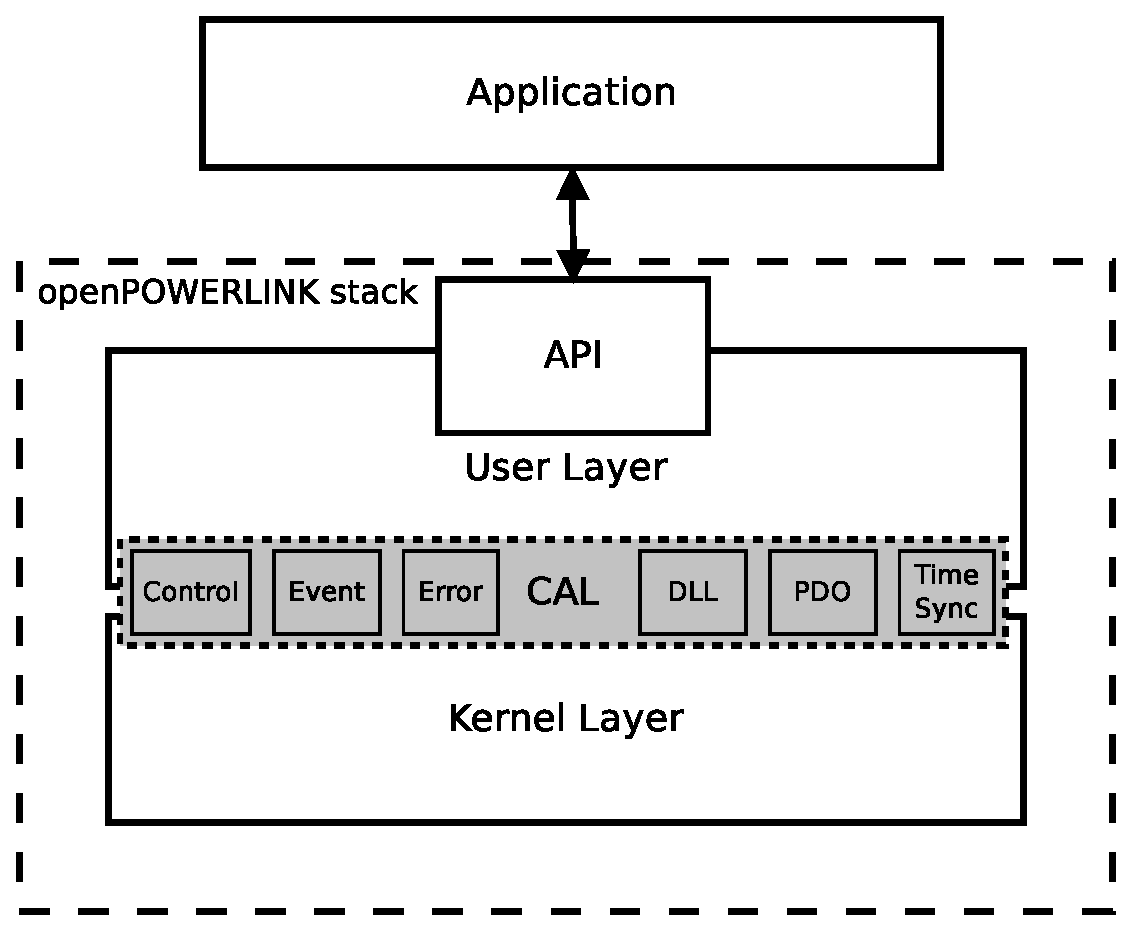
\includegraphics[width=1.2\textwidth]{../../thesis/images/openpowerlink_arch.eps}}
            \end{figure}
        \end{column}
    \end{columns}
\end{frame}

\begin{frame}{Platform Dependency}
    Realized via common header files and platform specific implementations.
    \newline
    
    
    \begin{block}{Implemented modules for minimal dependency}
        \begin{description}
            \item[target] General target specific functionalities (Led, IP Address, Default Gateway, Tickcount, sleep)
            \item[edrv] Ethernet driver
            \item[hrestimer] High resolution timer
            \item[sdoudp] Asynchronous data transmission via UDP
            \item[trace] Trace output for debugging
        \end{description}
    \end{block}
\end{frame}

\begin{frame}{Simulation}
    Separation of simulation and openPOWERLINK stack.
    
    
    \tikzoverlay[text width=6.5cm] at (5cm,-6cm) {
        \tikz node (label) at (0,0)[]{
            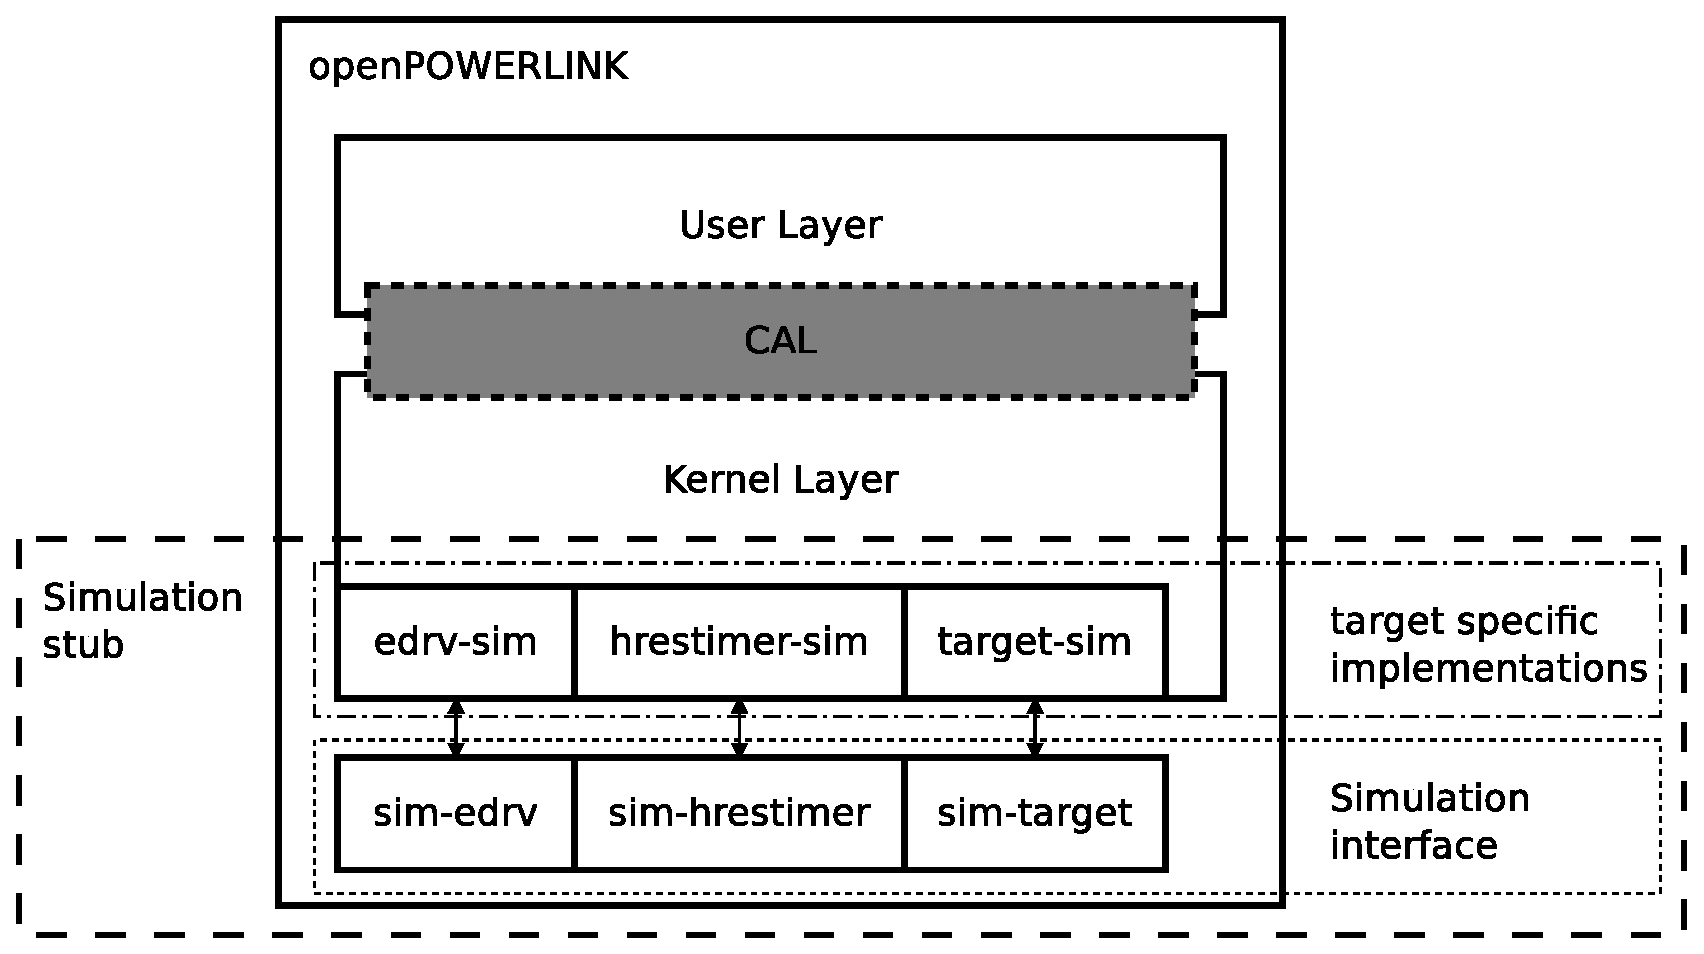
\includegraphics[width=1\textwidth]{../../thesis/images/simulation_stub.eps}
        };
    };
    \begin{block}{Simulation Stub}
        \begin{itemize}
            \item Target-specific implementations
            \begin{itemize}
                \item Implementation of platform dependent modules for \emph{sim} target
                \item Connection to simulation interface
                \newline
            \end{itemize}
            
            \item Simulation interface
            \begin{itemize}
                \item Connection to simulation\\
                environment (independent\\
                of OMNeT++)
                \item Calling stored function\\
                pointer with instance\\
                handle
            \end{itemize}
        \end{itemize}
    \end{block}
    
\end{frame}